\documentclass[10pt,twocolumn,letterpaper]{article}

\usepackage{cvpr}
\usepackage{times}
\usepackage{epsfig}
\usepackage{graphicx}
\usepackage{amsmath}
\usepackage{amssymb}
\usepackage{float}
\usepackage{graphicx,times}
\usepackage{subfigure}   
\usepackage{booktabs}  
\usepackage[UTF8]{ctex}

% Include other packages here, before hyperref.

% If you comment hyperref and then uncomment it, you should delete
% egpaper.aux before re-running latex.  (Or just hit 'q' on the first latex
% run, let it finish, and you should be clear).
\usepackage[breaklinks=true,bookmarks=false]{hyperref}

\cvprfinalcopy % *** Uncomment this line for the final submission

\def\cvprPaperID{****} % *** Enter the CVPR Paper ID here
\def\httilde{\mbox{\tt\raisebox{-.5ex}{\symbol{126}}}}

% Pages are numbered in submission mode, and unnumbered in camera-ready
%\ifcvprfinal\pagestyle{empty}\fi
\setcounter{page}{1}
\begin{document}

%%%%%%%%% TITLE
\title{作业1,2,3实验报告}

\author{Author\\
Chi Zhang 张弛\\
SJTU\\
{\tt\small 517021910658}
% For a paper whose authors are all at the same institution,
% omit the following lines up until the closing ``}''.
% Additional authors and addresses can be added with ``\and'',
% just like the second author.
% To save space, use either the email address or home page, not both
}

\maketitle
%\thispagestyle{empty}

%%%%%%%%% ABSTRACT

%%%%%%%%% BODY TEXT
\section{作业一}


\subsection{\textbf{任务一:高斯滤波}}

\textbf{从二维连续高斯函数中计算不同大小的高斯卷积模板(3*3,5*5, 7*7, 9*9, 11*11, 17*17);把卷积模板归一化;利用各个大小不一的高斯卷积模板对同一灰度图像进行卷积滤波,显示滤波后的图像结果,并从这些结果中总结高斯不同大小模板的图像滤波特点(观察细节、轮廓线的变化)}

二维高斯滤波的计算公式为:
\begin{equation}
   H_{i,j}=\frac{1}{2\pi\sigma^2}e^{-\frac{(i-k-1)^2+(j-k-1)^2}{2\sigma^2}}
\end{equation}
其中$(i,j)$为像素的位置,窗口模板的大小定义为$(2k+1)*(2k+1)$,$\sigma$为标准差参数,该值越小则生成的模板中心系数越大,周围系数越小,也就是平滑效果越明显。最终需要在模板的前面加一个系数,使得权值之和为1.

由题意得,计算大小为(3*3,5*5, 7*7, 9*9, 11*11, 17*17)的高斯模板,并将结果展示于图中~\ref{fig:matrix1}~\ref{fig:matrix2}~\ref{fig:matrix3}。

由此可以算出在不同的滤波模板下,处理图像的结果。选取其中一张图片,将其在不同滤波模板下的所有输出进行对比,展示于图中~\ref{fig:GaussScaleAll}。
为了更加直观地观测高斯滤波的效果,单独选取3*3与17*17两种高斯卷积模板滤波后的图像进行对比,其对比如图~\ref{fig:GaussScale2}。

总结高斯不同大小模板的图像滤波特点(观察细节、轮廓线的变化):随着滤波模板窗口的不断加大,图像细节缺失越严重,且轮廓线也越不清晰。图像整体表现趋于模糊。

\begin{figure}[th]
   \centering
   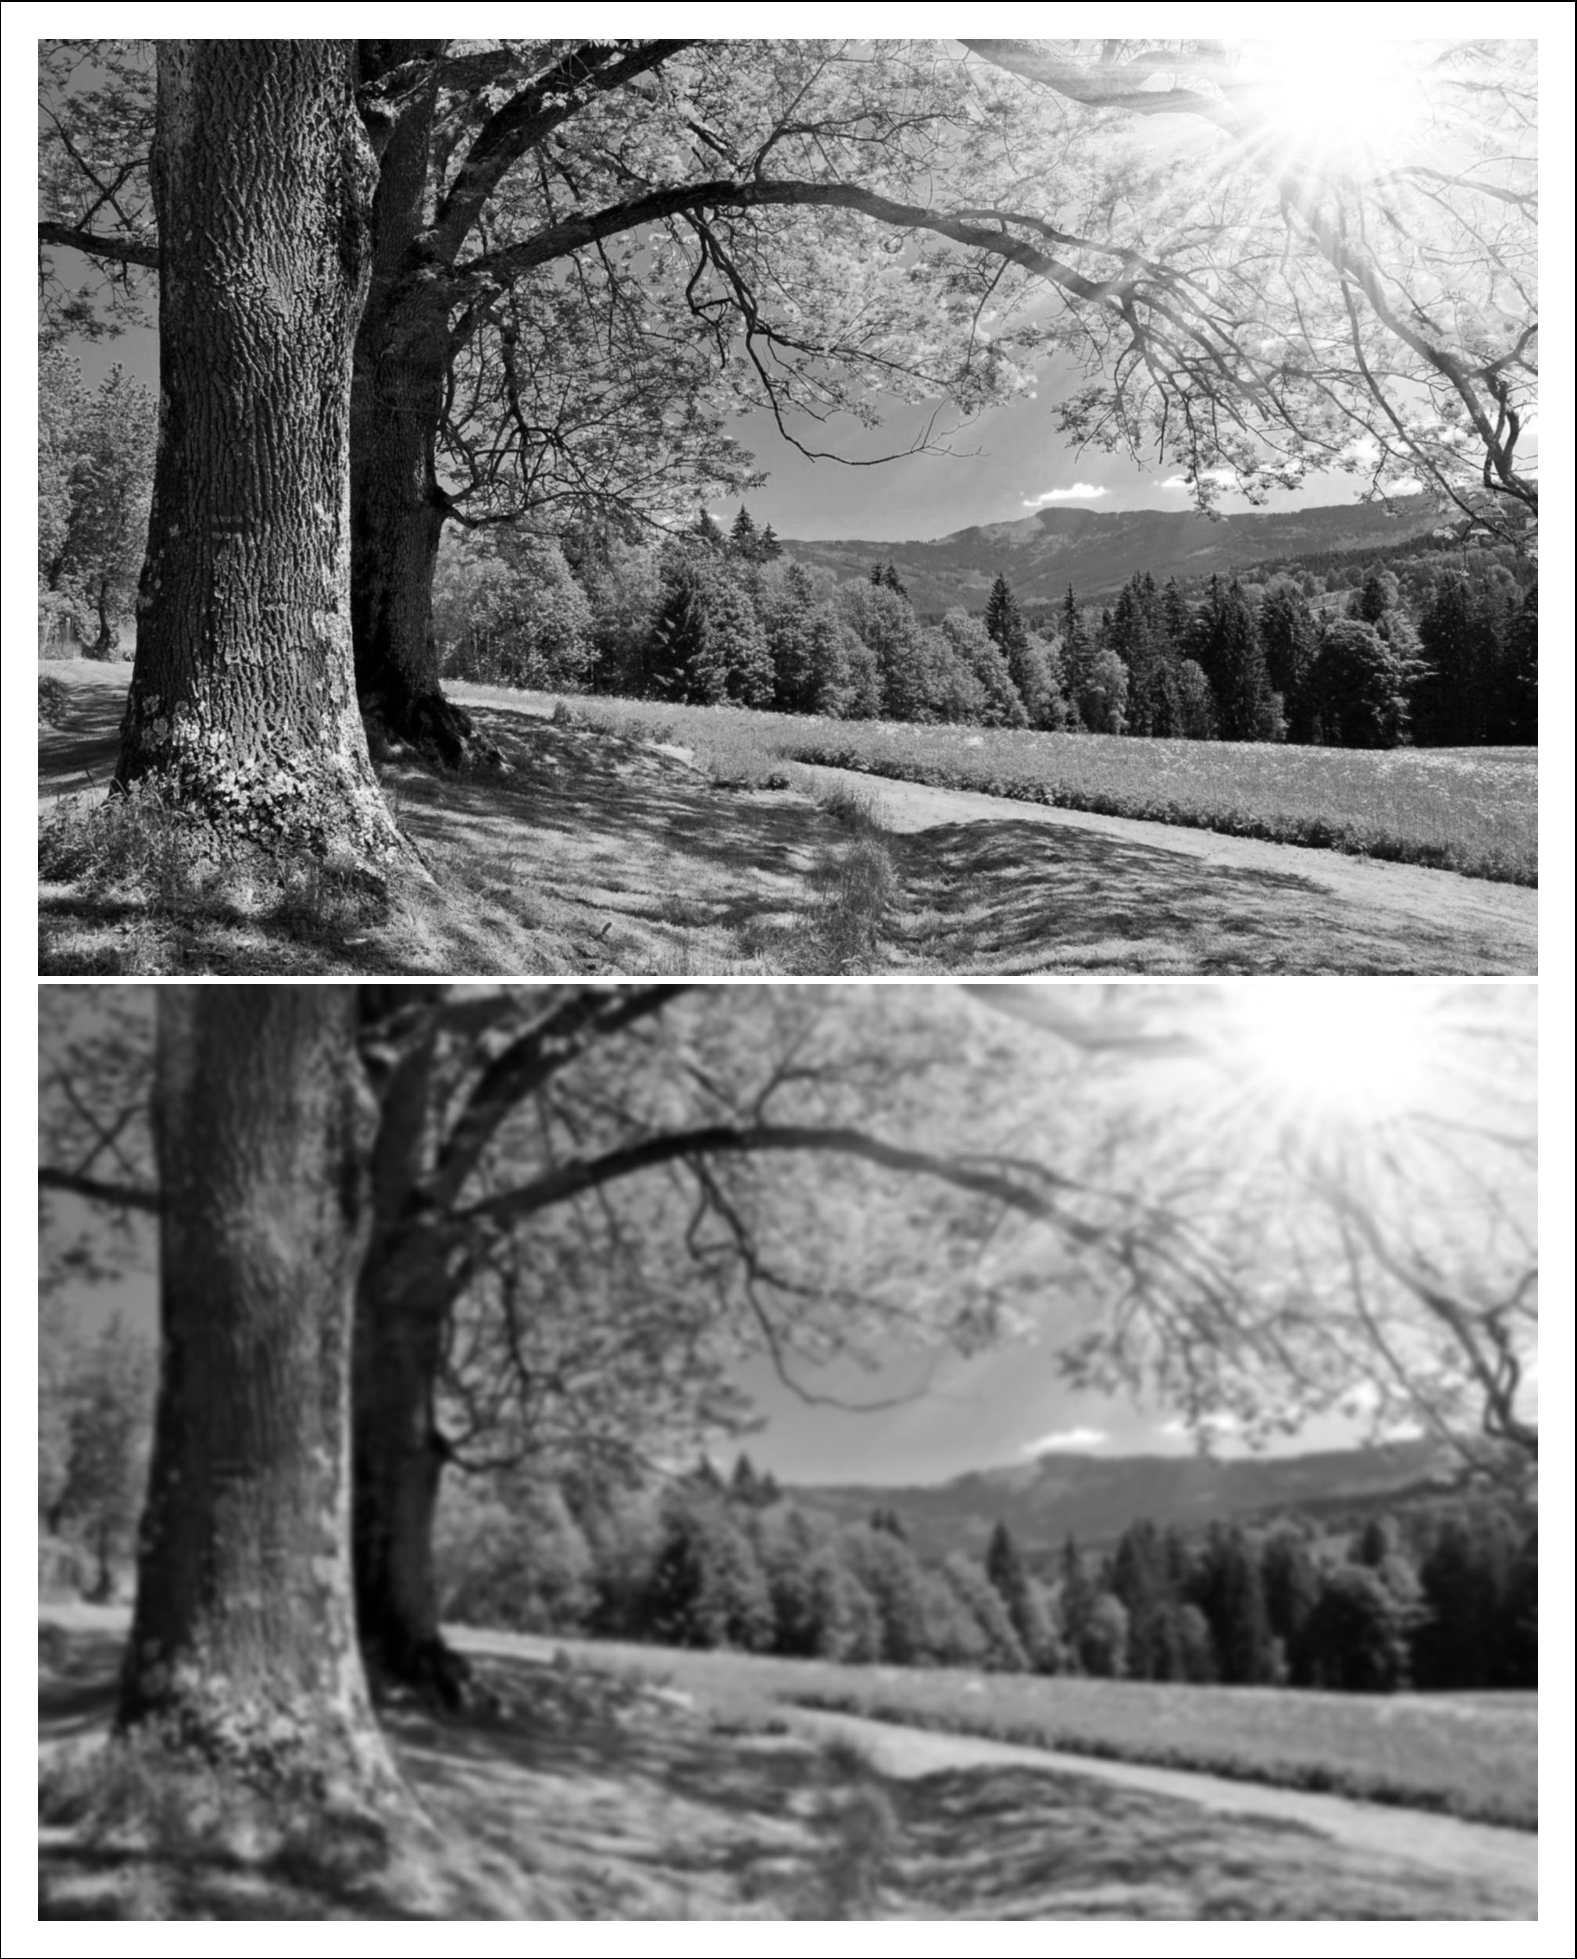
\includegraphics[width=0.95\linewidth]{GaussScale2.pdf}
   \caption{高斯卷积多尺度滤波后的图像。卷积模板:上为3*3,下为17*17}   
   \label{fig:GaussScale2}
\end{figure}


\clearpage


\begin{figure*}[th]
   \centering
   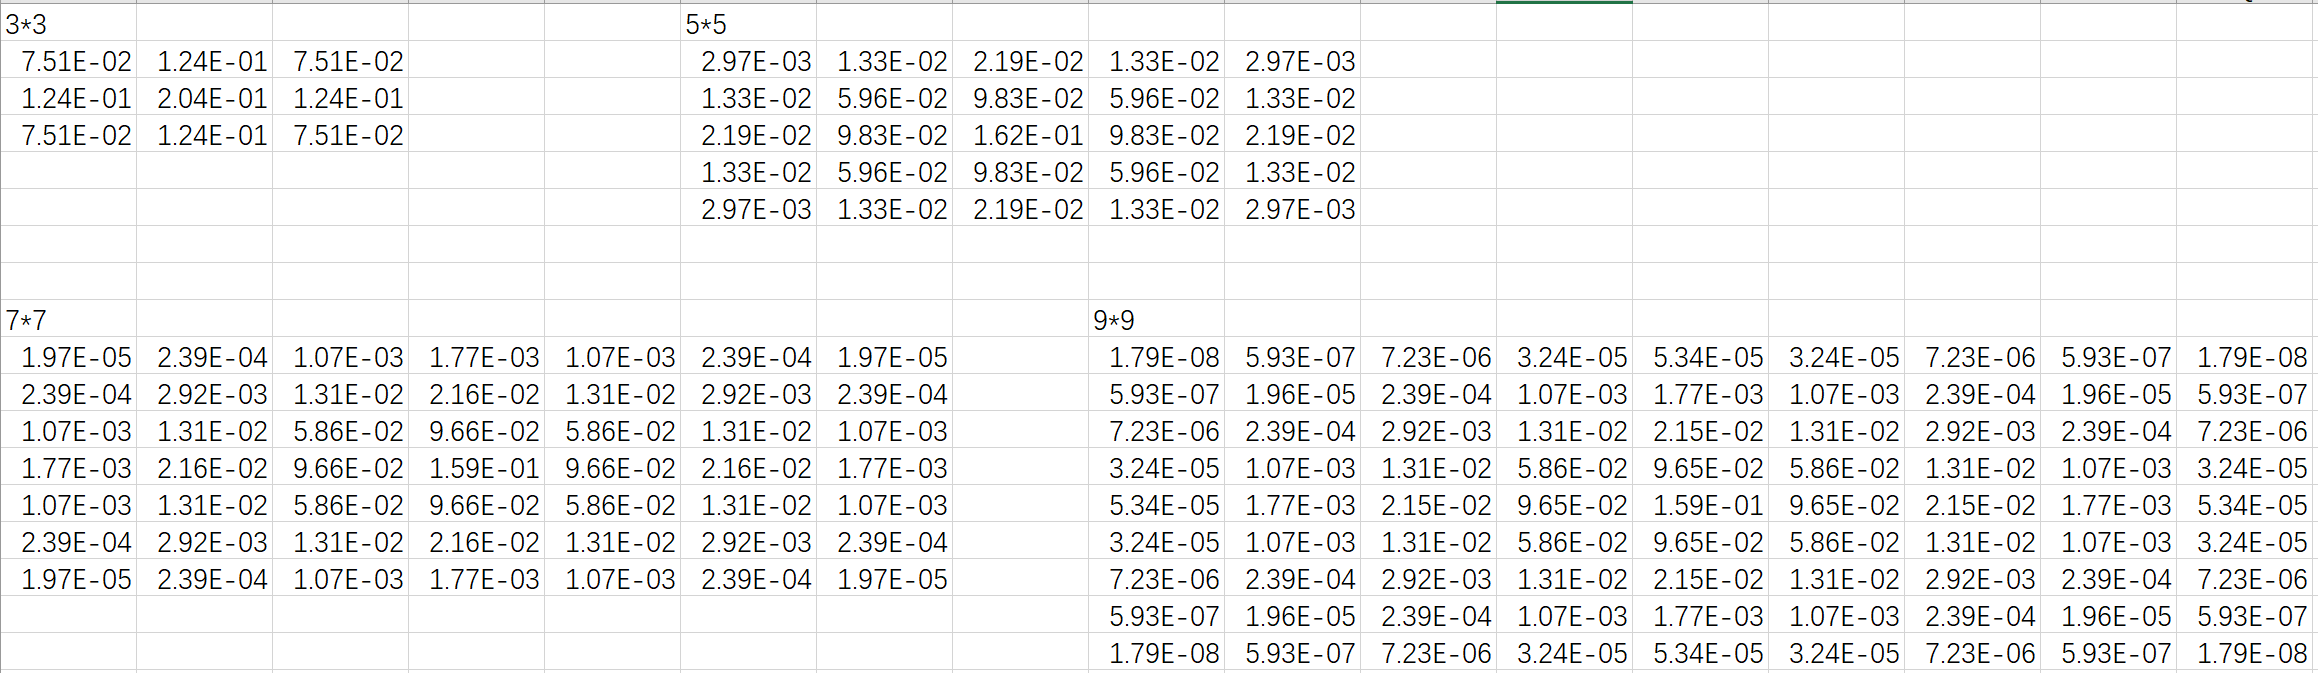
\includegraphics[width=0.95\linewidth]{matrix1.png}
   \caption{高斯卷积多尺度滤波的模板元素权重,包含3*3,5*5,7*7,9*9 的模板。}   
   \label{fig:matrix1}
\end{figure*}

\begin{figure*}[th]
   \centering
   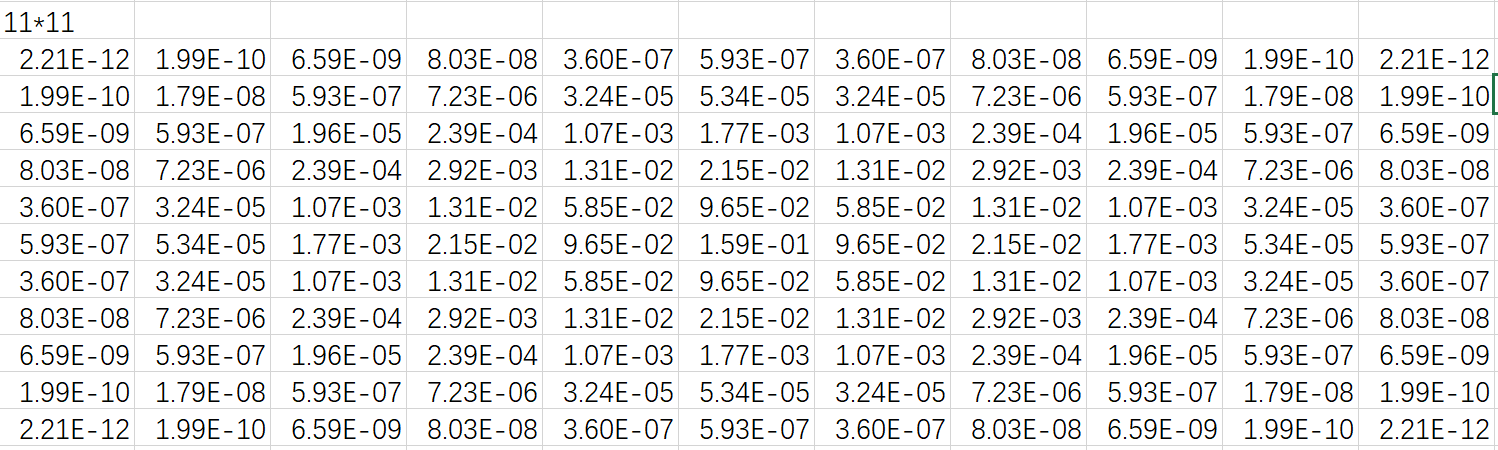
\includegraphics[width=0.95\linewidth]{matrix2.png}
   \caption{高斯卷积多尺度滤波的模板元素权重,包含11*11 的模板。}   
   \label{fig:matrix2}
\end{figure*}

\begin{figure*}[th]
   \centering
   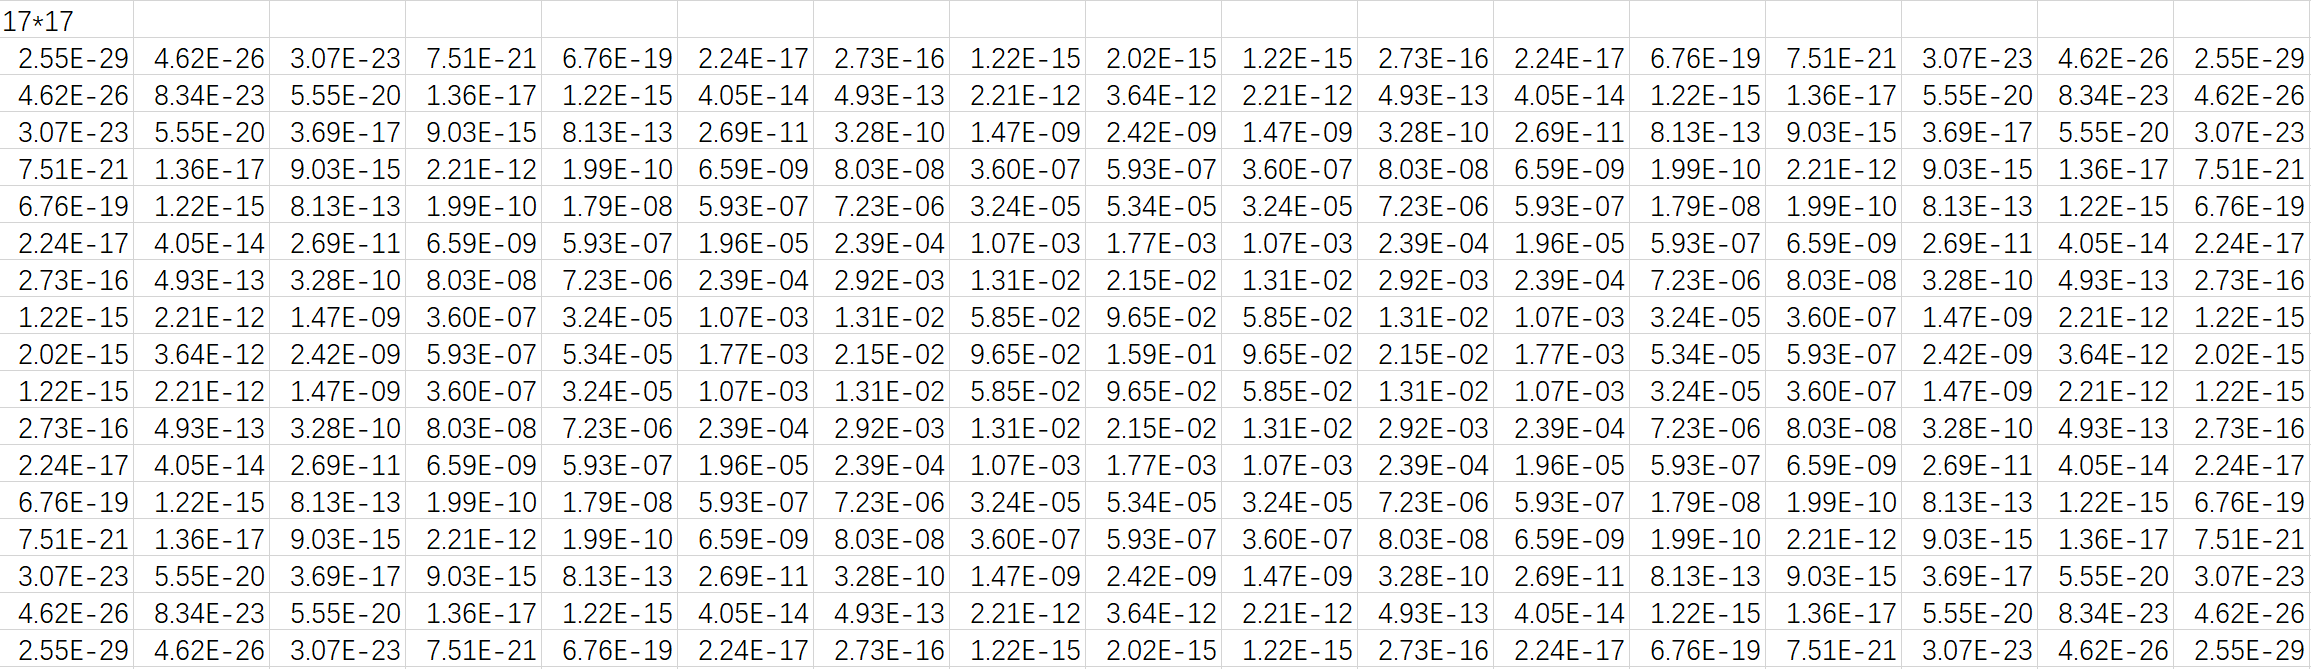
\includegraphics[width=0.95\linewidth]{matrix3.png}
   \caption{高斯卷积多尺度滤波的模板元素权重,包含17*17 的模板。}   
   \label{fig:matrix3}
\end{figure*}

\clearpage

\begin{figure*}[th]
   \centering
   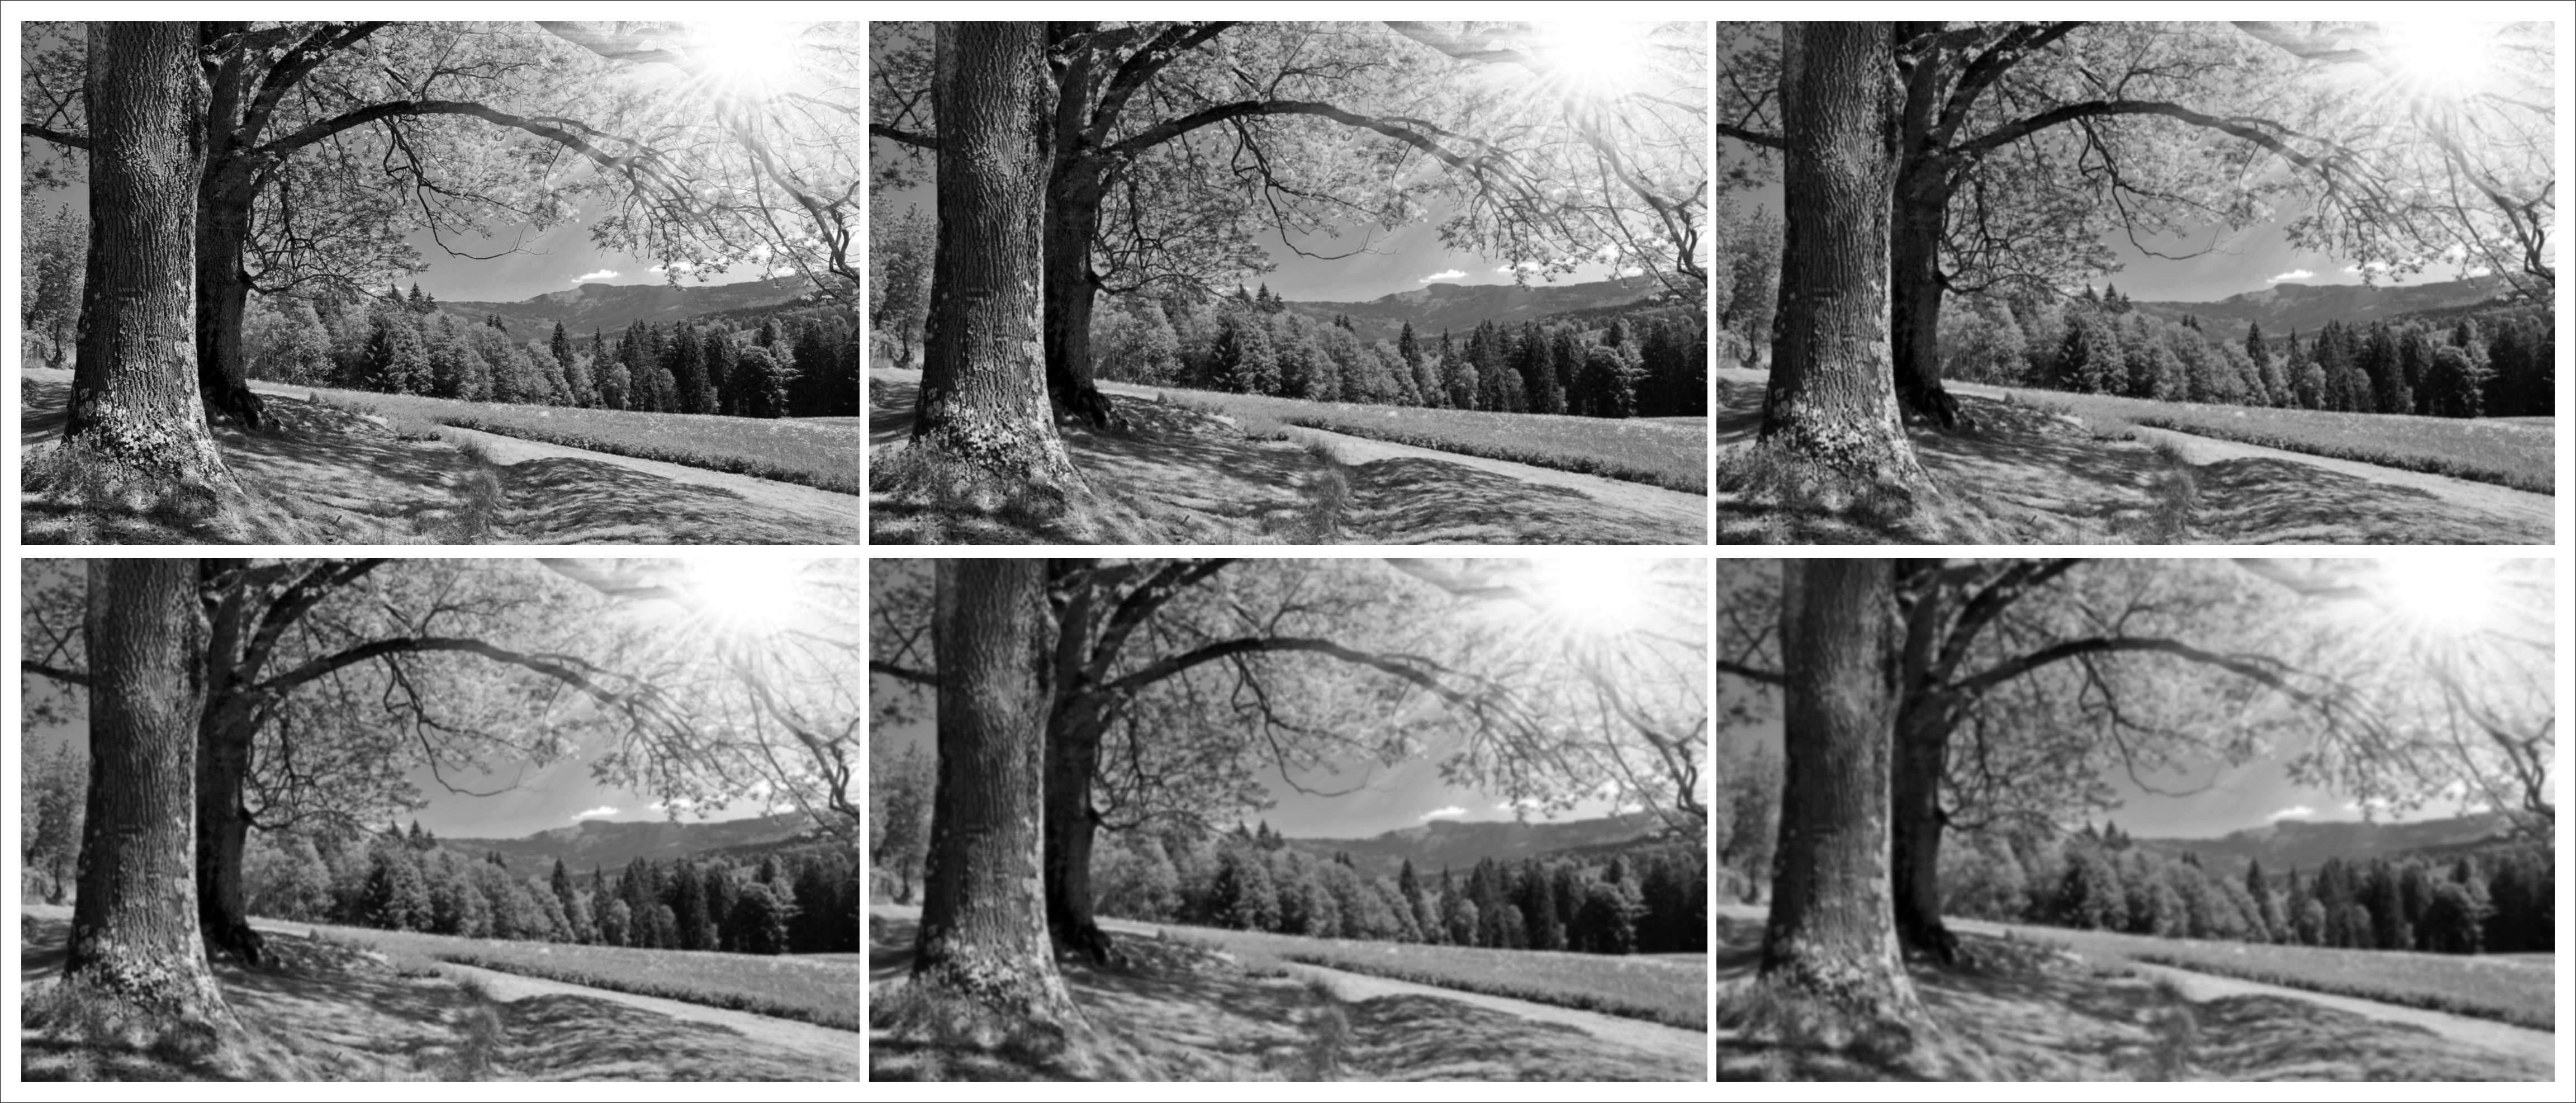
\includegraphics[width=0.95\linewidth]{GaussScaleAll.pdf}
   \caption{高斯卷积多尺度滤波后的图像。卷积模板:上从左到右为3*3,5*5,7*7,下从左到右为9*9, 11*11, 17*17}   
   \label{fig:GaussScaleAll}
\end{figure*}



\begin{figure*}[th]
   \centering
   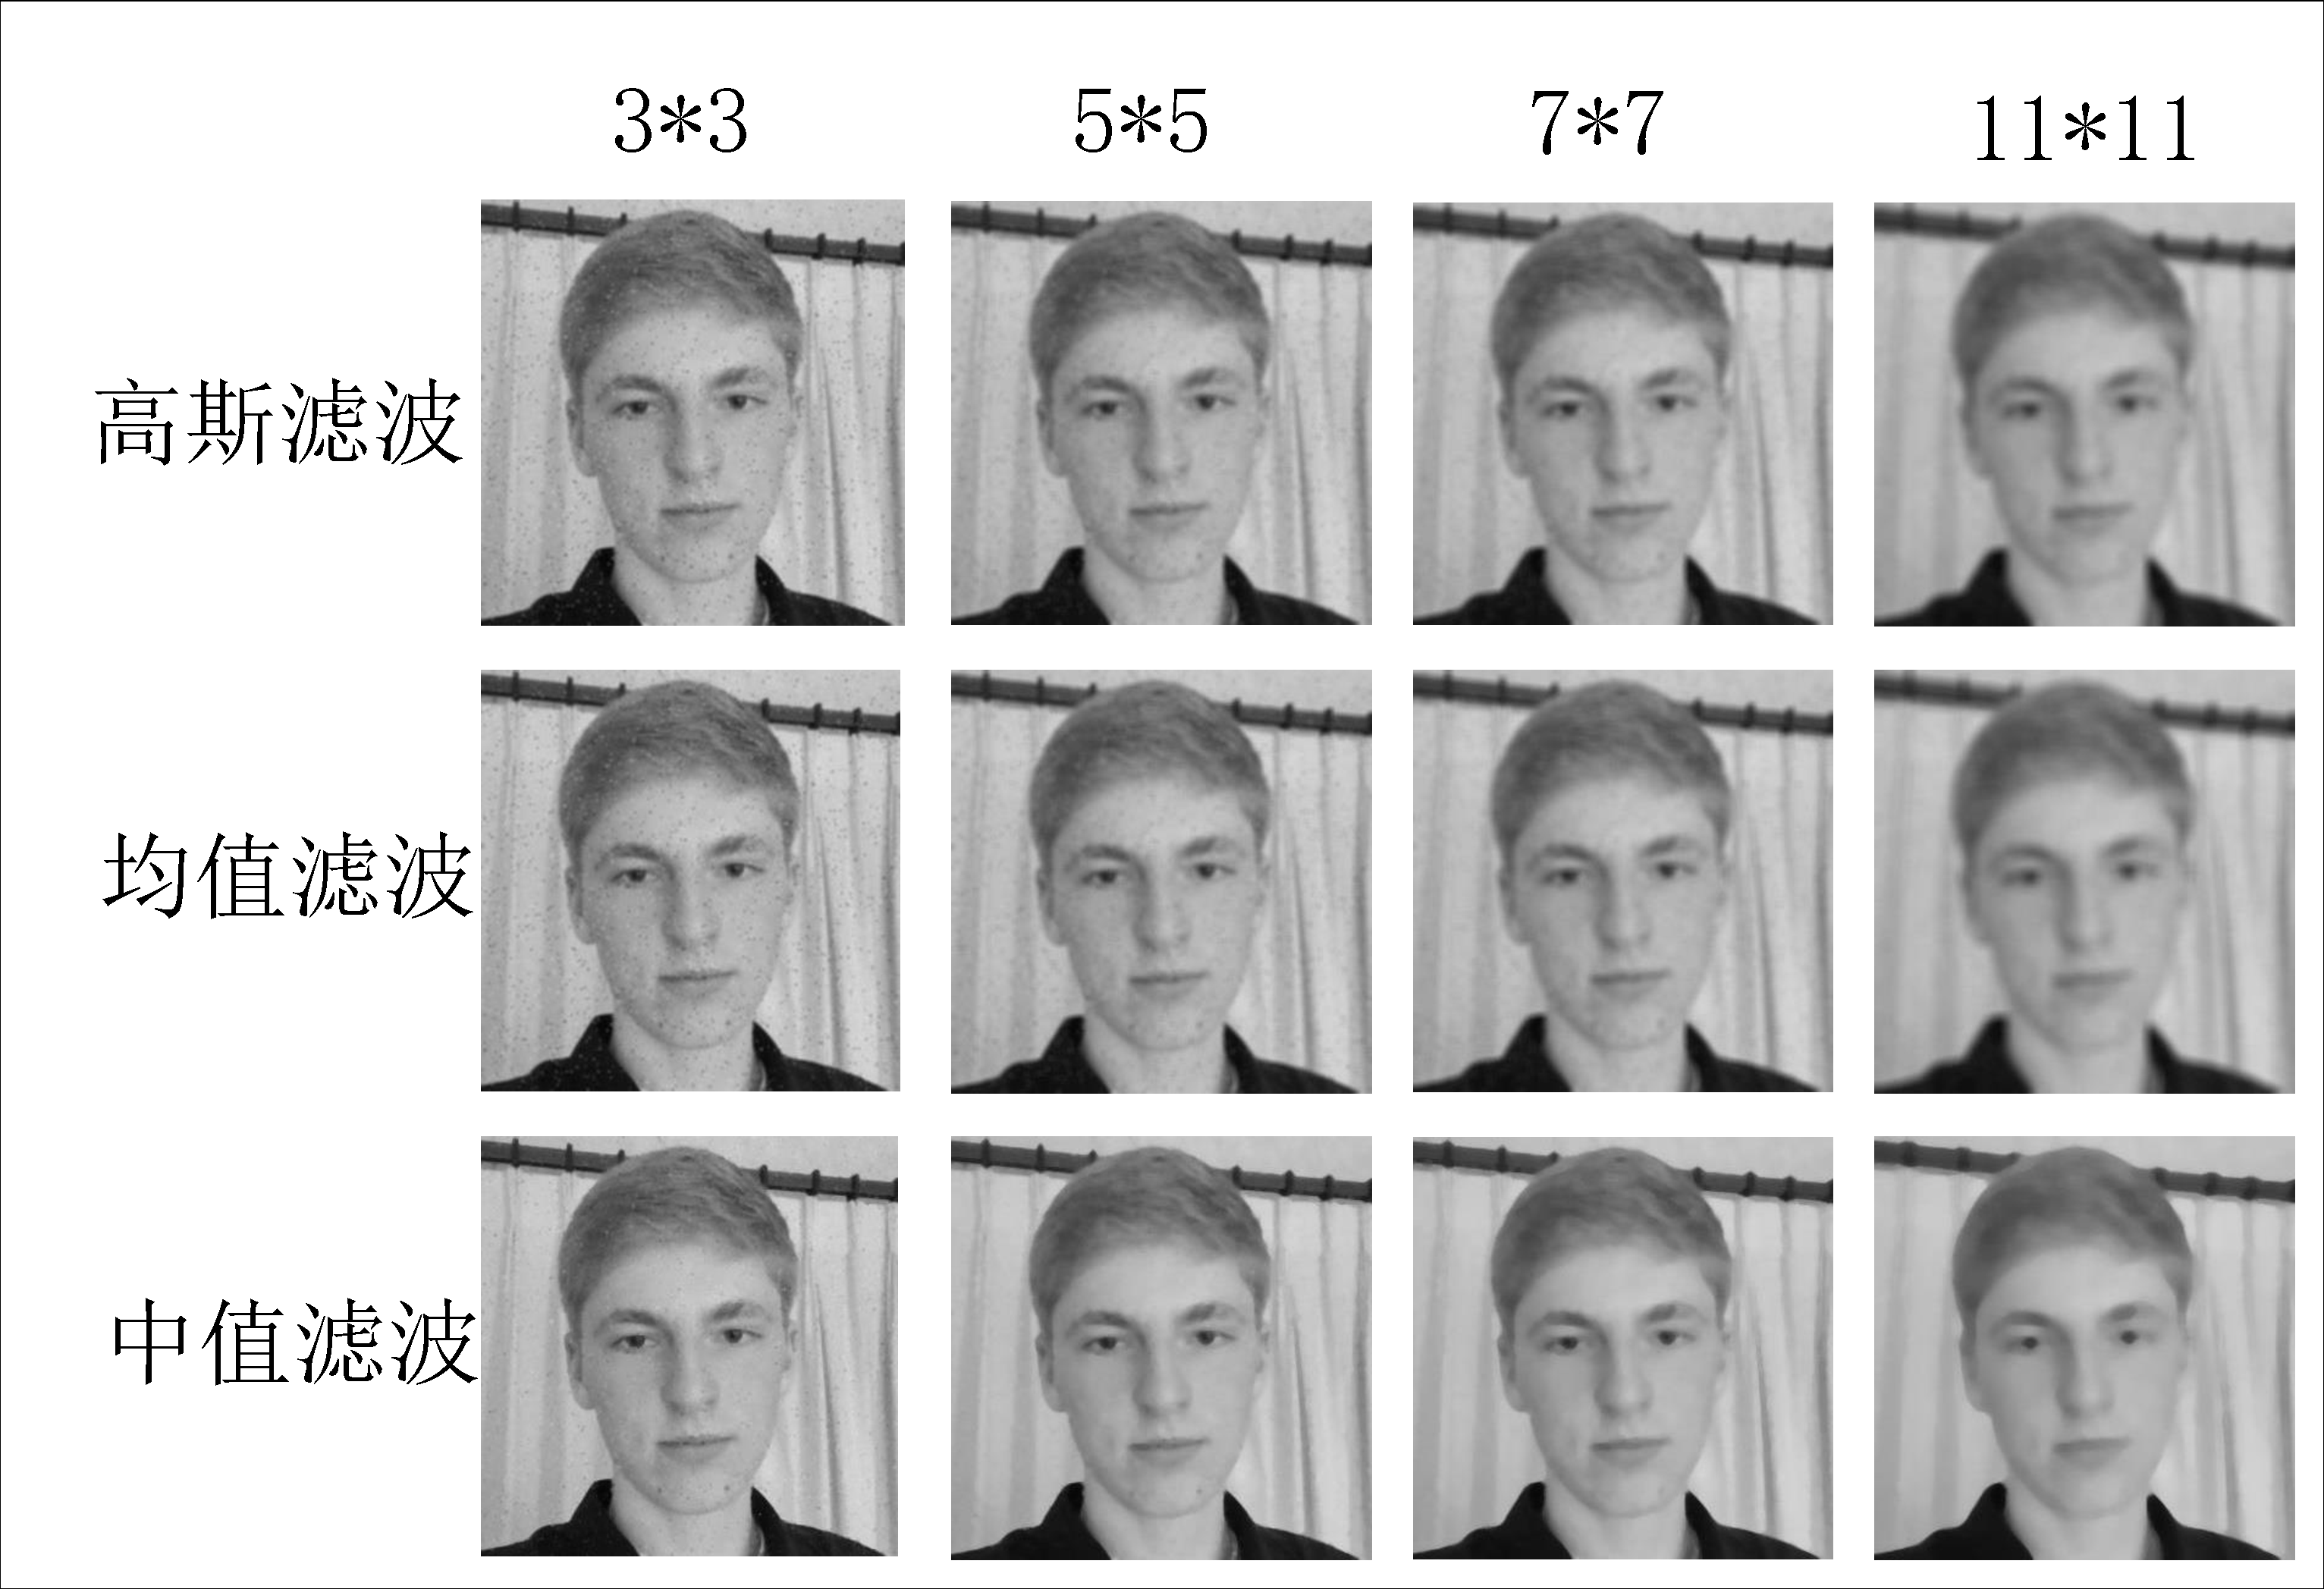
\includegraphics[width=0.95\linewidth]{GaussNoise2.pdf}
   \caption{高斯噪声图像在各类滤波器处理后的结果对比。}   
   \label{fig:GaussNoise1}
\end{figure*}

\begin{figure*}[th]
   \centering
   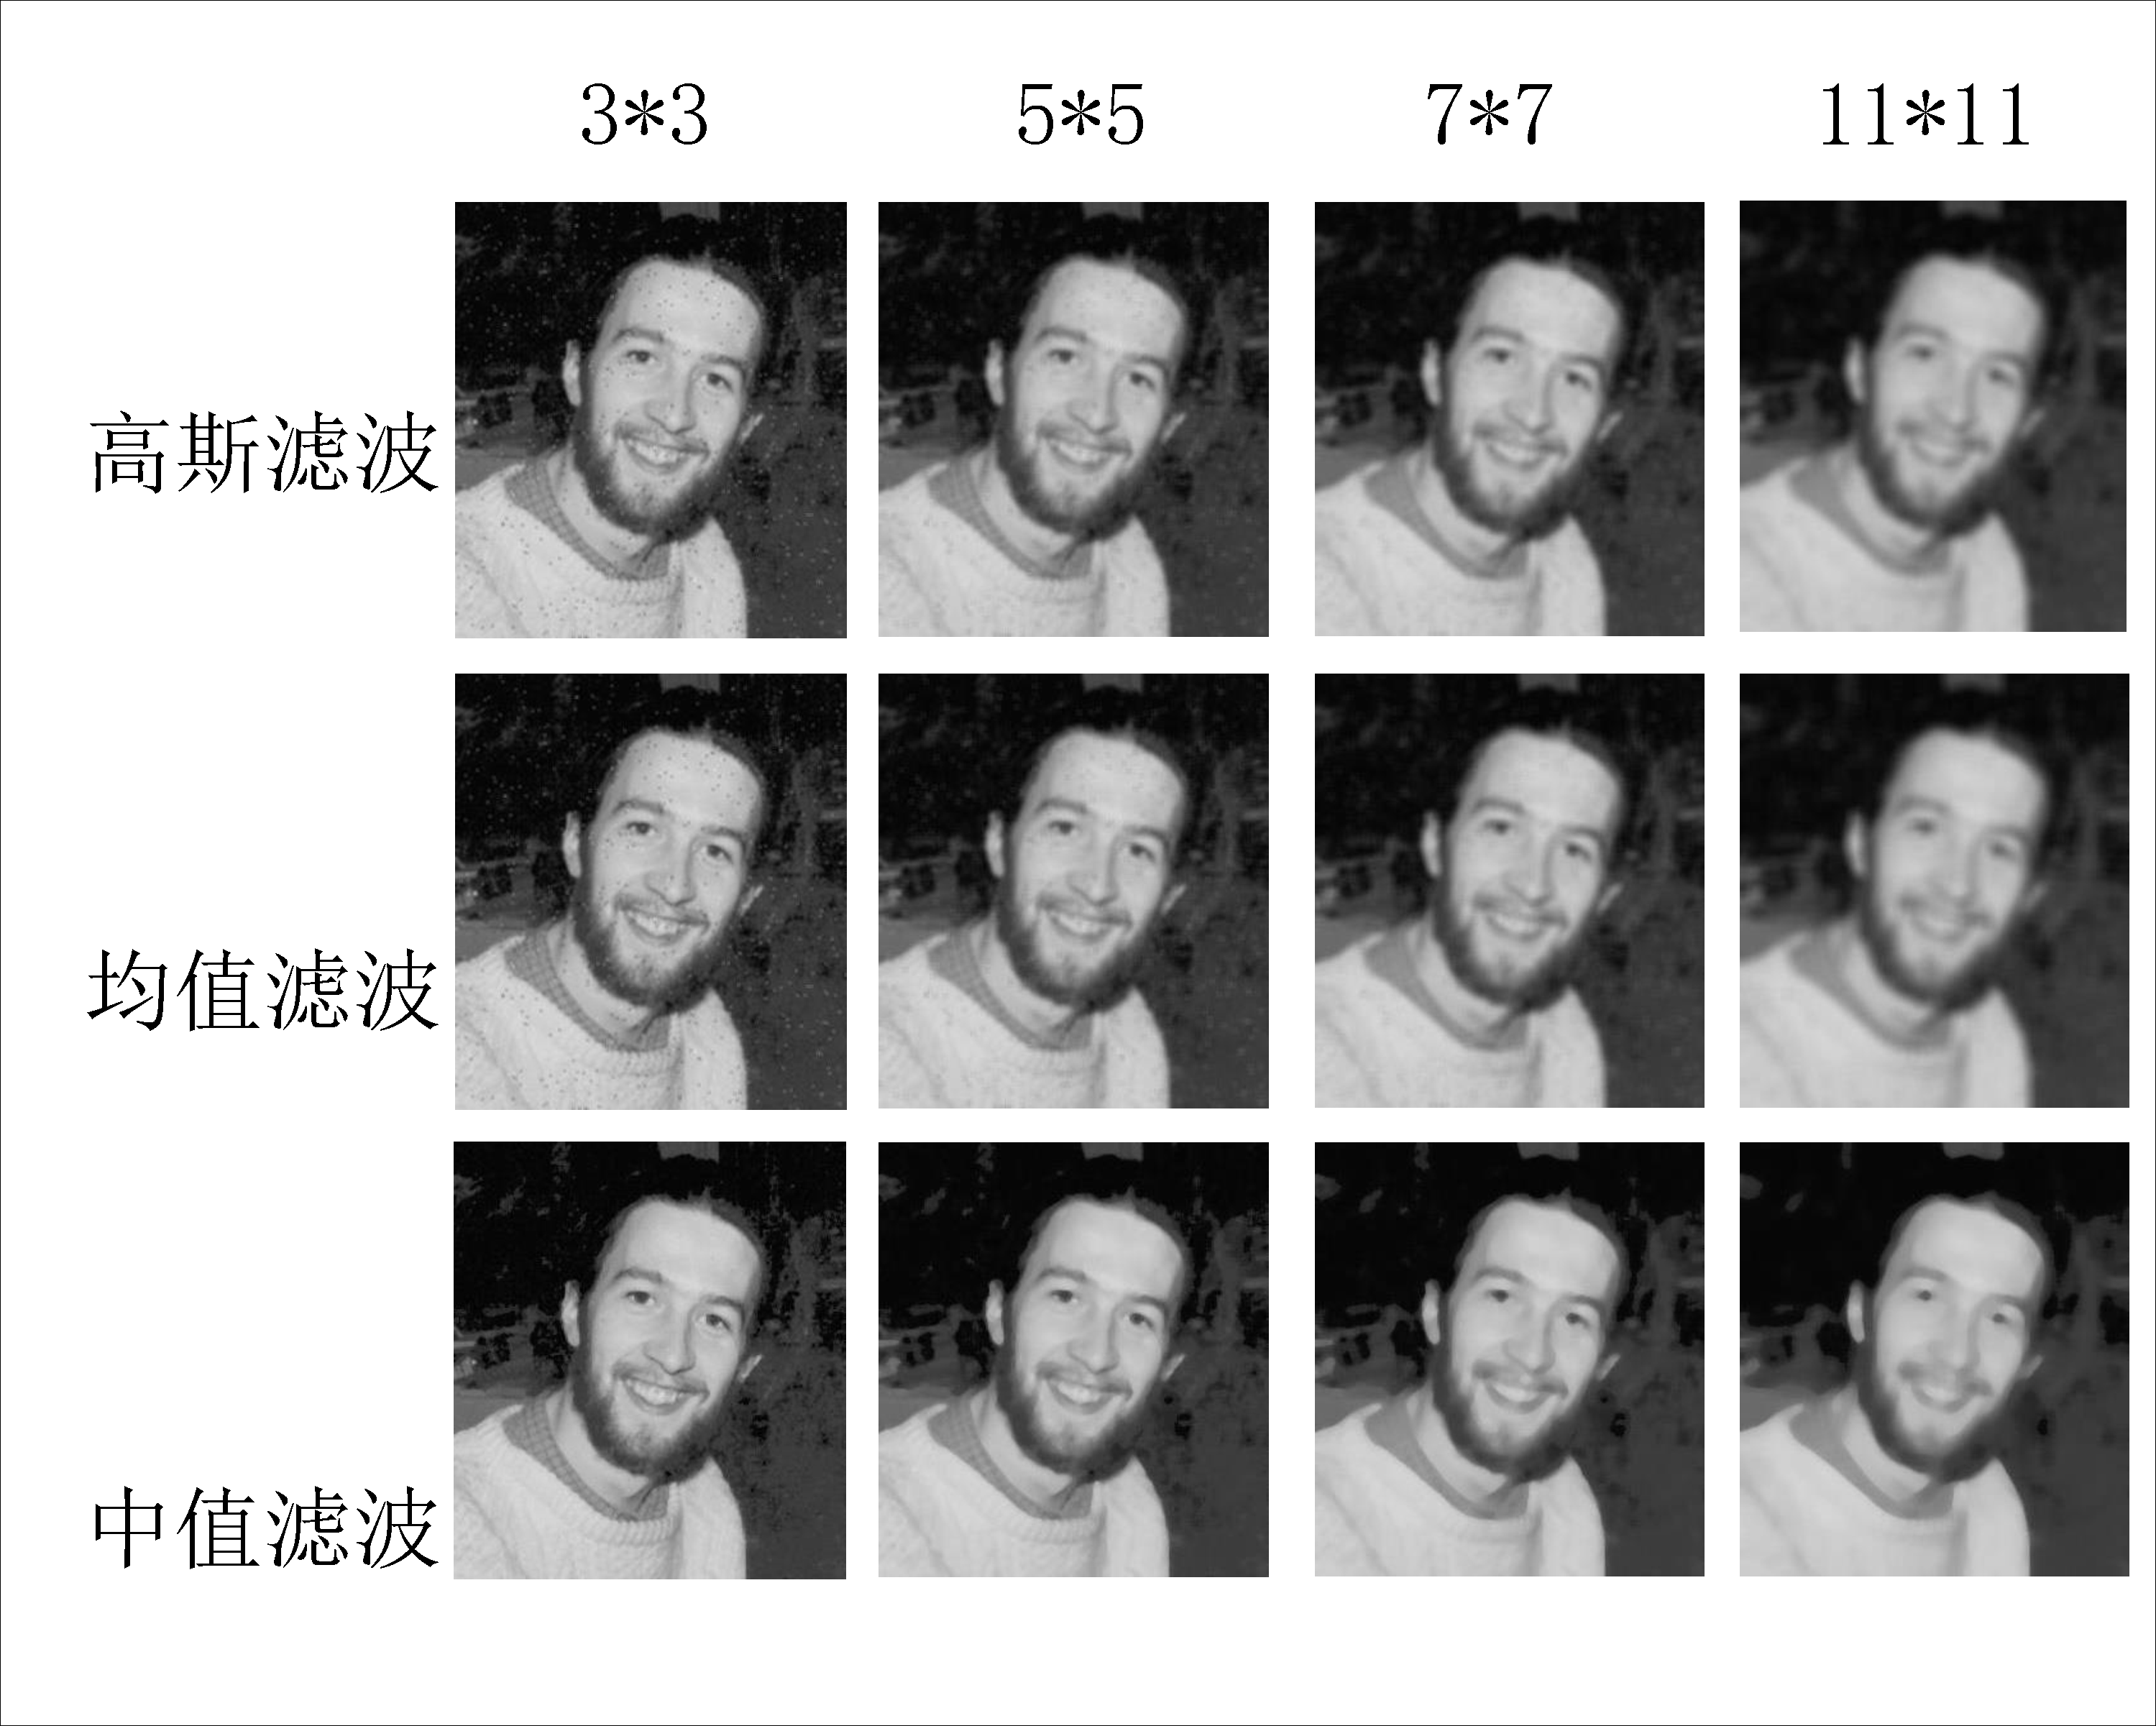
\includegraphics[width=0.95\linewidth]{SAPNoise1.pdf}
   \caption{椒盐噪声图像在各类滤波器处理后的结果对比。}   
   \label{fig:SAPNoise1}
\end{figure*}


\section{作业二}

\subsection{任务一:噪声滤波}

\textbf{程序实现并观察均值滤波子、中值滤波子、高斯滤波子在不同模板大小的情况下(3*3, 5*5, 7*7, 11*11;中值滤波考虑对应的不同的邻域)对噪声图像的滤波结果。总结一下模板大小变化时带来的特点}

对于包含不同噪声的图像,分别用(3*3, 5*5, 7*7, 11*11)的均值滤波子、中值滤波子、高斯滤波子进行滤波处理,得到处理后的图像。对于高斯噪声与椒盐噪声的图像,分别选取一张,展示各类滤波器处理图像的结果于图中~\ref{fig:GaussNoise1},~\ref{fig:SAPNoise1}。

\textbf{滤波模板大小对比}:对于任何图像,不论是何种滤波器,随着滤波模板窗口的不断加大,图像细节缺失越严重,且轮廓线也越不清晰。图像整体表现趋于模糊。

重点观测噪声点:可以发现当模板较小时,各类噪声点仍然较多,而当加大模板窗口的尺度,图像中的噪声点逐渐减少。

\textbf{滤波模板类型对比}:
\begin{itemize}
   \item 对于包含高斯噪声的图像,使用中值滤波最能有效地去除离群噪声点,其次是高斯滤波,而均值滤波的效果最差。但不论是哪种滤波方式,在模板窗口较小时,仍有较多噪声点未被去除,但随着窗口加大,噪声点去除的同时图像本身的信息与细节也被模糊,因此这些滤波方式在面对高斯噪声时效果并不显著。
   
   重点观测噪声点:对于高斯噪声,当滤波器尺度较小时各类滤波器的除噪效果并不是都很明显,只有中值滤波器能实现部分的除噪,而高斯滤波和均值滤波保留了大部分噪声点。

   \item 对于包含椒盐噪声的图像,使用中值滤波能非常有效地去除离群点,3*3的中值滤波模板就能有效地滤除大部分噪声点。而高斯滤波与均值滤波效果均一般,低尺度的滤波模板几乎不能去除噪声点。
   
   重点观测噪声点:对于椒盐噪声,当滤波器尺度较小时只有中值滤波器能实现较好的除噪,而高斯滤波和均值滤波保留了大部分噪声点。
\end{itemize}

\subsection{任务二:理想滤波子}
\textbf{理想的噪声滤波可以描述为:在去除噪声的同时,不影响图像中的内容(主要指轮廓线、图像细节等)。解释一下理想滤波子为什么难以实现。}

滤波器会产生振铃效应。由卷积定理可知,频率域下的理想低通滤波器$H(u, v)$必定存在一个空间域下与之对应的滤波函数$h(x, y)$,且可以通过对$H(u,v)$作傅里叶逆变换求得。产生振铃效应的原因在于,理想低通滤波器在频率域下的分布十分线性(在D0处呈现出一条垂直的线,在其他频率处呈现出一条水平的线),对应的$h(x,y)$将会有类似于$sinc$函数那样周期震荡的空间分布特性。正是由于理想低通滤波器的空间域表示有类似于$sinc$函数的形状,位于正中央的突起使得理想低通滤波器有模糊图像的功能,而外层的其他突起则导致理想低通滤波器会产生振铃效应。通俗地说,滤波去除噪声与保留图像细节信息两者是不可兼得的,去除噪声的同时势必会影响图像中的内容,使得轮廓线模糊,图像细节流失,理想滤波子难以实现。振铃效应几乎不可避免,尤其对于有噪声存在的场合,它会混淆图像的高频特性,使得振铃效应带来的影响更加显著。

\clearpage

\section{作业三}

\subsection{任务一:图像梯度}
\label{sec:greetings}
\textbf{数字图像中如何计算梯度?}
图像是离散函数,在某点的梯度可以用向前差商、向后差商或者中心差商获得。

图像$f(x,y)$在位置$(x,y)$的梯度定义为向量
$$ \nabla F=
\left[
    \begin{array}{c}
        G_x \\
        G_y \\
    \end{array}
\right]
=
\left[
    \begin{array}{c}
        \frac{\partial f}{\partial x} \\
        \frac{\partial f}{\partial y} \\
    \end{array}
\right]
$$

$$
\nabla f = mag(\nabla F) = [G_x^2+G_y^2]^{\frac{1}{2}}
$$

$$
a(x,y)=arctan_y(\frac{G_y}{G_x})
$$

\begin{itemize}
   \item Roberts 交叉梯度算子:   
   $$
   \nabla f  \approx |G_x|+|G_y|=|z_9-z_5|+|z_8-z_6| 
   $$

   \item Prewitt梯度算子:  
   \begin{multline*}
      \nabla f  \approx |G_x|+|G_y|=|(z_7+z_8+z_9)-(z_1+z_2+z_3)| \\
      +|(z_3+z_6+z_9)-(z_1+z_4+z_7)|
   \end{multline*}

   \item Sobel梯度算子:  
   \begin{multline*}
      \nabla f  \approx |G_x|+|G_y|=|(z_7+2z_8+z_9)-(z_1+2z_2+z_3)| \\
      +|(z_3+2z_6+z_9)-(z_1+2z_4+z_7)|
   \end{multline*}


\end{itemize}

\subsection{任务二:度量灰度变化}
\textbf{如何度量局部区域灰度的变化?}

在图像中物体边缘处,灰度值变化幅度较大;而物体内部,灰度值变化幅度较小。计算图像的梯度可以定量地反映局部区域的灰度变化程度。在上文~\ref{sec:greetings} 中对各种梯度算子进行了介绍总结。

\subsection{任务三:噪声中的灰度变化}
\textbf{如何在有噪声的情况下合理估算局部区域灰度的变化?}

有以下两种思路,在有噪声的情况下合理估算局部区域灰度的变化。
\begin{itemize}
   \item 平滑去除噪声。
   
   利用高斯滤波器、均值滤波器、中值滤波器等方法,先对图像进行平滑滤波处理,除去噪声点。这样的缺点是会使得图像轮廓线和细节模糊,使信息流失。

   \item 抑制噪声的梯度算子。
   
   计算梯度时,合理选择梯度算子能有效抑制噪声的影响。例如Sobel算子模板对噪声有较强的鲁棒性。
\end{itemize}

%{\small
%\bibliographystyle{ieee_fullname}
%\bibliography{egbib}
%}

\end{document}
